\chapter{Test Setups}
\label{chap:\currfilebase}

\subsection{Hammer-Hammer Test}

The hammer tips of the reference system and the experimental system are hit against eachother.
\\[4ex]
\begin{minipage}{\linewidth}
\centering
\begin{minipage}[b]{0.7\textwidth}
    \centering
    \includestandalone[scale=0.7]{\imgpath/test_setups/HH_parts/HH_parts}
    \captionof{figure}[Hammer-Hammer Test components]{Hammer-Hammer test components}
    \label{fig:HH_parts}
\end{minipage}
\hspace{0em}
\begin{minipage}[b]{0.2\textwidth}
    \centering
    \footnotesize
    \def\circlabel#1#2{%
        \begin{tikzpicture}[%
            x=1em,y=1ex,
            baseline={([yshift=3] N.south)},
            font={\fontsize{6pt}{6.2pt}\selectfont},
            ]%
            \node[%
                circle, fill=white, draw=#1, line width=1pt,
                inner sep=2pt, minimum size=8pt, align=center,
                ] (N) {#2};
        \end{tikzpicture}
    }
    \begin{tabular}{c@{ :\hskip 0.5em}l}
        \toprule
        \large{\circlabel{WesMixL8qual3}{1}} & Piezo + \acs{AMP}\\
        \large{\circlabel{WesMixL8qual3}{2}} & Soft Tip\\
        \large{\circlabel{WesMixL8qual3}{3}} & Tip 34CrMo4\\
        \large{\circlabel{WesMixL8qual3}{4}} & \acs{LC} DYMH-103\\
        \large{\circlabel{WesMixL8qual3}{5}} & \acs{IN-AMP} AD627\\
        \bottomrule
    \end{tabular}
    \normalsize
    \captionof{table}[Legend to Hammer Hammer Test Components]{Legend to \figref{fig:HH_parts}}
    \label{tab:HH_parts}
\end{minipage}
\end{minipage}\\[4ex]

\begin{figure}[!htb]
    \centering
    \includestandalone[width=0.9\linewidth]{\imgpath/test_setups/HH_comparison/HH_comparison}
    \caption[HH-Test comparison]{The HH-Test recordings of the reference hammer (orange) and the evaluated impact hammer system (turquoise). Note that the evaluated signal values are normalized so that the maxima are equal to the reference system.}
    \label{tab:mcu_com_protocol}
\end{figure}
\begin{figure}[!htb]
    \centering
    \includestandalone[width=\linewidth]{\imgpath/test_setups/HH_noise/HH_noise}
    \caption[HH-Test comparison]{The HH-Test recordings of the reference hammer (orange) and the evaluated impact hammer system (turquoise). Note that the evaluated signal values are normalized so that the maxima are equal to the reference system.}
    \label{fig:HH_noise}
\end{figure}

\subsection{Andromeda FRF measurement}

\begin{figure}[!htb]
    \centering
    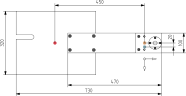
\includegraphics[scale=1]{\imgpath/test_setups/Andromeda/Andromeda_Positions_Top}
    \caption[Andromeda Positions Top View]{Andromeda}
    \label{Andromeda_Positions_Top}
\end{figure}

\begin{figure}[!htb]
    \centering
    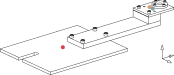
\includegraphics[scale=1]{\imgpath/test_setups/Andromeda/Andromeda_Positions_Trimetric_coord}
    \caption[Andromeda Positions Trimetric View]{Andromeda}
    \label{Andromeda_Positions_Trimetric_coord}
\end{figure}

\begin{figure}[!htb]
    \centering
    \includegraphics[width=0.5\linewidth]{\imgpath/test_setups/Andromeda/Andromeda_Sensors.jpg}
    \caption[Andromeda Positions Sensors View]{Andromeda}
    \label{Andromeda_Sensors}
\end{figure}

% \begin{figure}[!htb]
%     \centering
%     \includegraphics[width=0.5\linewidth]{\imgpath/test_setups/Andromeda/Andromeda_total.jpg}
%     \caption[Andromeda Overview]{Andromeda_total}
%     \label{Andromeda_total}
% \end{figure}